\documentclass[10pt,letterpaper]{report}
\usepackage{enumitem}
\usepackage[utf8]{inputenc}
\usepackage[spanish]{babel}
\usepackage{graphicx}
\usepackage{amsmath}
\usepackage{amsfonts}
\usepackage{amssymb}
\usepackage{makeidx}
\usepackage[usenames]{color}
\usepackage[left=2cm,right=2cm,top=1.5cm,bottom=1.5cm]{geometry}
\usepackage{subfiles}
\usepackage[ruled, vlined, lined, linesnumbered, algochapter, spanish]{algorithm2e}
\usepackage{longtable}
\usepackage{tikz}
\usetikzlibrary{babel}
\usetikzlibrary{positioning}
\usetikzlibrary{decorations.pathreplacing,arrows.meta,calc}
\usepackage{float}



\SetKwInput{Entrada}{Entrada}
\SetKwInput{Salida}{Salida}

\SetKwIF{If}{ElseIf}{Else}
{Si}{hacer}
{sino si}{sino}{}

\SetKw{Devolver}{Devolver}

\SetKwFor{ForEach}{Para cada}{hacer}{}

\SetKwFor{While}{Mientras}{hacer}{fin mientras}

\definecolor{Micolor1}{RGB}{255,0,0}

% titlesec para personalizar capítulos
\usepackage{listings}
\usepackage{xcolor}
\usepackage{titlesec}

\lstset{
    language=Java,
    basicstyle=\ttfamily\small,
    keywordstyle=\color{blue}\bfseries,
    stringstyle=\color{red},
    commentstyle=\color{green!50!black},
    numbers=left,
    numberstyle=\tiny,
    stepnumber=1,
    numbersep=8pt,
    showspaces=false,
    showstringspaces=false,
    frame=single,
    breaklines=true,
    inputencoding=utf8,
    extendedchars=true,
    literate=
        {á}{{\'a}}1
        {é}{{\'e}}1
        {í}{{\'i}}1
        {ó}{{\'o}}1
        {ú}{{\'u}}1
        {ñ}{{\~n}}1
        {Ñ}{{\~N}}1
}

\titleformat{\chapter} % Configuración de capítulos
	{\Large\bfseries}	% formato del texto
	{\huge \thechapter}	% número grande
	{20pt}				% espacio
	{\huge}				% formato del título

% Numeración de ejemplos por capítulo
\newtheorem{problema}{Problema}[chapter]

\begin{document}

\begin{center}
    \begin{minipage}{3cm}
    	\begin{center}
    		\includegraphics[height=3.4cm]{logo_unam.png}
    	\end{center}
    \end{minipage}\hfill
    \begin{minipage}{10cm}
    	\begin{center}
    	\textbf{\large Universidad Nacional Autónoma de México}\\[0.1cm]
        \textbf{Facultad de Ciencias}\\[0.1cm]
        \textbf{Modelado y Programación $|$ Grupo 7079}\\[0.1cm]
        Proyecto: Base de Datos Musical \\[0.1cm]
        Erick Xavier Martinez Briones\\[0.1cm]
        13 de Noviembre de 2026
    	\end{center}
    \end{minipage}\hfill
    \begin{minipage}{3cm}
    	\begin{center}
    		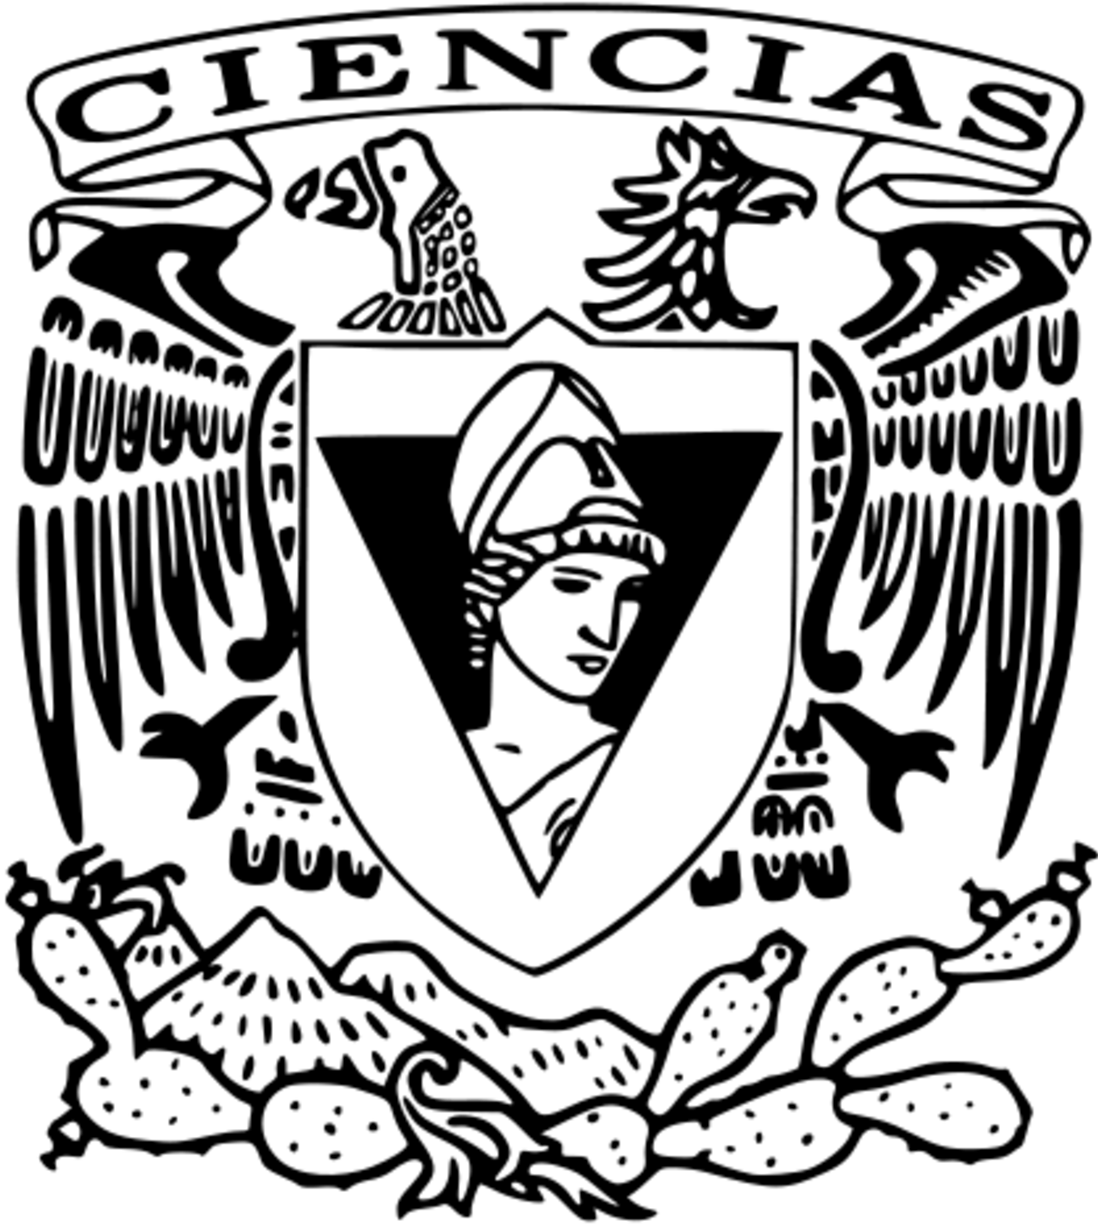
\includegraphics[height=3.4cm]{Logo_FC.png}
    	\end{center}
    \end{minipage}
\end{center}

\rule{17cm}{0.1mm}

\begingroup
  \let\clearpage\relax
  \let\cleardoublepage\relax

\begin{center}
{\Large\bfseries Resumen}
\end{center}

\begin{quote}
El problema a resolver es el desarrollo de un sistema gestor de archivos de formato mp3; este problema se atacará siguiendo el proceso de la cascada del desarrollo de software el cuál se expondrá a lo largo de este reporte de proyecto. El núcleo de este sistema orbita alrededor de un nuevo concepto como lo son las bases de datos, las cuales nos van a permitir la persistencia de datos en el sistema, además de que tambien está presente el tema del desarrollo de interfaces de usuario que permiten una interacción amigable con el sistema, por ello es que durante el desarrollo del reporte se encontrarán las justificaciones a las decisiones que se tomarón para la elaboración de este software, como lo pueden ser el uso de distintos patrones de diseño, asi como el uso de tecnológias particulares como pueden ser Qt o .NET incorporado al lenguaje C\#, el cual es el lenguaje principal en el que se desarrollo este software.
\end{quote}
  
  \chapter{Introducción al problema}

\noindent  Al seguir avanzando en la materia \textit{Modelado y Progrmación}, nos vmemos en la necesidad de realizar un nuevo proyecto para que, de esa manera, nuestro conocimiento sobre el proceso de desarrollo de software se vaya puliendo; por lo anterior, tenemos que como segundo proyecto a realizar, el desarrollo de un software encargado de gestionar archivos con formato mp3 usando una base de datos. 

\vspace{0.2cm}

\noindent  Durante el implementación del primer proyecto, logramos dimensionar los factores que se involucran en el desarrollo de software; dicho conocimiento y aprendizaje, se deberá de ver reflejado en este nuevo proyecto, evitando cometer algunas de los fallas que entorpecen el desarrollo del proyecto.
\vspace{0.2cm}

\noindent El desarrollo de la aplicación nos presenta nuevas tecnologías con las cuales estaremos interactuando durante nuestra vida como programadores, estas herramientas son nuevas para mi, pues antes no habia trabajado con ellas de manera directa, por esto, es que el proyecto presenta de manera inherente dificultades a superar, pues nuevamente, es tener que aprender a usar (o al menos a tener las nociones básicas) de dichas tecnologías.
\vspace{0.2cm}

\noindent Algunas de las herramientas nuevas que presenta este proyecto es tener nociones de como trabajar usando una base de datos, pues tomando en cuenta el contexto del proyecto, al estar desarrollando un gestor de archivos mp3, la aplicación deberá tener acceso a los archivos mp3 del usuario y deberá poder almacenarlos en alguna entidad para poder hacer uso de ellos. La base de datos resuelve este problema, pues es el ente en donde podremos almacenar los datos de los archivos mp3 para poder tener persistencia de dichos datos.
\vspace{0.2cm}

\noindent Otra de las grandes herramientas que estan inmiscuidas en este proyecto, son las interfaces de usuario para poder tener una interacción amigable entre el usuario y la computadora. Durante nuestra formación como computólogos, hemos desarrollado interfaces para poder interactuar con nuestros programas, pero en su mayoria son interfaces hechas en la terminal de nuestros equipos, esto esta bien para las necesidades que requerimos en su momento, pero no es de extrañar que un usuario común al ver una terminal abierta piense que es el nuevo Anonymous, pues no es la forma en que se interactua de manera común con un programa; el problema anterior, de generar una interacción amigable con el usuario, se resuelve haciendo un programa que contenga una interfaz gráfica para el usuario (GUI), que no es algo que se debe de tomar a la ligera, pues más alla de las dificultades técnicas ``comúnes`` que se pueden presentar, (como problemas de compilación, sintáxis etc), se presentan dificultades como lo son la creatividad que se puede llegar a tener para realizar una GUI atractiva y hasta cierto punto intuitiva para un usuario, que en principio no debería de conocer todas las funcionalidades que tiene nuestro programa.
\vspace{0.2cm}

\vspace{0.2 cm}

\noindent Los puntos mencionados previamente solo son algunos de los retos a los cuales nos enfrentaremos al desarrollar este programa, pero son estos retos los que nos permiten seguir ampliando nuestra visión como programadores, de esa manera, dichos retos deberán tener un correcto plan de ataque para poder resolverlos de la manera más optima posible, dicho plan estará plasmado en este reporte, pues como vimos en el proyecto anterior, al analizar los problemas que se nos presentan antes de actuar, encontrar soluciones, analizar dichas solucionres, y en general, tener una etapa de modelado sólida, nos ayudará a poder reaccionar de mejor manera a los retos que se nos presenten durante la etapa de implementación

\vspace{0.2cm}




    \chapter{Análisis del problema}


\noindent Hemos definido el problema resolver, ahora deberemos de analizar como llegar a una solución factible. En primera instancia, deberemos de preguntarnos si el problema es computable. Esta parte no requiere tanto análisis pues podemos decir de manera segura que en efecto lo es, pues el problema se puede resolver con una serie de pasos bien definifidos además de que se pueden completar en tiempo finito; vemos que el sistema de gestor de archivos mp3, requiere uso de operaciones que se pueden modelar como algortimos, que de primera impresión resultan no ser demasiado complejos, pues puede haber algoritmos como \textit{ObtenerTodasLasCancionesDelDirectorio} o \textit{EditarNombreDelArchivo} (solo por poner algunos ejemplos) que en conjunto resuelvan el problema planteado, de esa manera vemos que el problema que nos están dando si es computable.

\vspace{0.5cm}

\noindent Bien, una vez definido lo anterior, vale la pena aplicar de nueva cuenta la técnica de ``Divide y vencerás``, pues nuestro problema puede albergar muchos subproblemas que deberemos tomar en cuenta. Para abordar dichos retos, yo considero que no nos debemos de casar completamente con la idea de hacer un desarrollo ``Bottom Up`` o ``Top Down``, que si bien, sería lo ideal, pues tendriamos una linea estricta la cuál seguir, esto puede llegar a ser complejo, pues constantemente tendriamos que ir regresando en el análisis pues habrá omisiones que no tomamos en cuenta, por lo tanto, lo plantearemos de la siguiente forma:

\begin{itemize}
    \item Haremos uso de la técnica ``Top Down`` para plantear la arquitectura de sistema, es decir, haremos la separación de los modulos de los cuales se compondrá nuestro sistema, para de esa manera manejar de forma adecuada la separación de responsabilidades.
    \item La técnica ``Bottom Up`` la aplicaremos para dar forma y funcionalidad a cada modulo que definamos.
\end{itemize}

\noindent De esa manera, vemos que el desarrollo lo haremos de manera hibrida, pues haremos uso de ambas técnicas para poder obtener el sistema de gestor de archivos. Esta solución me parece adecuada, pues es hasta cierto punto intuitiva, y me parece que asi abarcamos de mejor manera los subproblemas que podremos llegar a encontrar. 

\noindent De hecho, considero que es intuitiva, pues incluso podemos aplicar una analogía: Veamos a todo el sistema de gestor de archivos mp3, como una casa, buscamos una manera de poder construirla, asi vemos que primero tiene sentido delimitar las cuartos que tendrá nuestra casa (estos son los modulos) además de que hay que tomar en cuenta que cada cuarto tiene una función en particular, pues no haces de comer en tu recámara o no duermes en el baño (esta es la separación de responsabilidades de cada módulo); lo anterior se ajusta a la estrategía Top Down, pues aquí es donde planeamos la arquitectura de la casa.

\noindent Una vez que ya tenemos delimitado cada cuarto, ahora hay que empezar llenar el cuarto para que cumpla su funcionalidad; supongamos por ejemplo la recamará, pensamos en cosas pequeñas, como los focos o contactos, después pensamos en agregar los muebles, las ventanas o en general cosas más grandes, que, en conjunto con las pequeñas proporcionan funcionalidad a la recámara; el paso anterior se ajusta a la estrategía Bottom Up, pues a partir de primero enfocarnos en los componentes más pequeños los integraremos progresivamente para que en su total, hagan posible el funcionamiento de cada módulo, que tambien a su vez, al integrarse todos los módulos, hagan posible el funcionamiento del sistema completo.


\vspace{0.5cm}

\noindent Asi que una vez que ya decidimos las estrategías que vamos a seguir, pasaremos a explicar cada una de ellas.

\vspace{0.5cm}

\noindent \textbf{Estrategía Top-Down para los módulos que integrarán nuestro sistema.}

\noindent Pensemos en las necesidades generales que necesita el sistema que nos proponen. Necesitamos un sistema de gestor de archivos mp3, llamemosle ``\textit{Reproductor Mp3}``, así que es lógico pensar que necesitamos un módulo que se encargue de alojar los datos de los archivos mp3, así que es el primer punto que nuestro sistema necesita.

\noindent Dicho módulo por ahora le llamaremos \textit{Informacion-Datos}

\begin{figure}[H]
\centering

\begin{tikzpicture}[
    box/.style={draw, rounded corners, align=center,
                text width=2.8cm, minimum height=1cm},
    >=latex
]

% Nodo principal
\node[box] (A) at (0,0) {Reproductor Mp3};

% Nodo hijo
\node[box] (B) at (0,-3) {Informacion-Datos};

% Conexión recta
\draw[->] (A) -- (B);

\end{tikzpicture}

\caption{Módulo Información-Datos}
\label{fig:informacion-datos}
\end{figure}

\vspace{0.5cm}

\noindent Una vez que ya tenemos resuelto donde alojar los datos que recuperamos de los archivos mp3, debemos pensar como es que nosotros vamos a obtener dichos datos, pues si bien el sistema no será encargado de descargar los archivos, pues ya estamos dando por supuesto que el usuario los tiene en su computadora, si es encargado de recuperar la información o metadada de dichos archivos, por tanto tiene sentido pensar en un módulo que se encargue de recuperar dicha información de los archivos mp3 que el usuario ingrese, al cuál le llamaremos \textit{Obtener-Información-Datos}.
\vspace{0.5cm}

\begin{figure}[H]
\centering

\begin{tikzpicture}[
    box/.style={draw, rounded corners, align=center,
                text width=2.8cm, minimum height=1cm},
    >=latex
]

% Nodo principal
\node[box] (A) at (0,0) {Reproductor Mp3};

% Nodos hijos en una fila
\node[box] (B) at (-2.2,-3) {Informacion-Datos};
\node[box] (C) at ( 2.2,-3) {Obtener-Informacion-Datos};

% Conexiones con codo
\foreach \n in {B,C}
    \draw[->] (A.south) -- ++(0,-0.8) -| (\n.north);

\end{tikzpicture}

\caption{Módulo Obtener-Informacion-Datos}
\label{fig:obtener-informacion-datos}
\end{figure}

\vspace{0.3cm}

\noindent Vemos que si bien, ambos modulos trabajan con los datos de los archivos mp3, estan separados, pues cada uno los maneja de manera distinta, pues mientras que un modulo maneja los archivos para obtener su metadata, el otro módulo solo se encarga de ser el ``recipiente`` en donde los vamos a alojar, es por ello que son módulos separados.

\noindent

\vspace{0.5cm}

\noindent Siguiendo con el análisis de aquellos compónentes generales que requiere nuestro sistema, debemos tomar en cuenta que un gestor de archivos mp3, más alla de solamente alojar los archivos, tambien es capaz de modificar la información que contiene cada uno de ellos, por tanto tener un módulo que se encargue exclusivamente de dicho fin nos ayudará a la solución del problema, llamaremos a dicho módulo \textit{Acceder-Información}

\vspace{0.5cm}

\begin{figure}[H]
\centering

\begin{tikzpicture}[
    box/.style={draw, rounded corners, align=center,
                text width=2.8cm, minimum height=1cm},
    >=latex
]

% Nodo principal
\node[box] (A) at (0,0) {Reproductor Mp3};

% Nodos hijos en una fila
\node[box] (B) at (-3.3,-3) {Informacion-Datos};
\node[box] (C) at ( 0,-3)   {Obtener-Informacion-Datos};
\node[box] (D) at ( 3.3,-3) {Acceder-Informacion};

% Conexiones con codo
\foreach \n in {B,C,D}
    \draw[->] (A.south) -- ++(0,-0.8) -| (\n.north);

\end{tikzpicture}

\caption{Módulo Acceder-Informacion}
\label{fig:acceder-informacion-2}
\end{figure}

\vspace{0.5cm}

\noindent Ahora bien, debemos de considerar que la información que vamos a estar manejando de cada archivo mp3 (que a partir de aquí lo vamos a generalizar a una canción) como puede ser su nombre, quienes son los interpretes, e incluso el mismo archivo, se pueden llegar a presentar de formas distintas dentro del propio sistema, pues dicha información la podremos llegar a ver como los metadatos del propio archivo, como información que se guarda dentro del módulo definido para ello o como elementos que el usuario veŕa en el producto final.

\vspace{0.2cm}

\noindent Si cada vez que una parte del sistema tuviera que definir por su cuenta dichos datos, tendríamos muchas formas de representar lo mismo, y un cambio en cualquiera de esas partes tendría que modificar a todas las demás, lo que es complicado. Por ello, es necesario que definamos a un módulo que se encargue de guardar dichas entidades, para que cada parte del sistema pueda tener compartir un acceso sin tener la necesidad de definirla por su cuenta, es por ello que a dicho módulo le llamaremos ``Entidades-compartidas``.

\vspace{0.5cm}
\begin{figure}[H]
\centering

\begin{tikzpicture}[
    box/.style={draw, rounded corners, align=center,
                text width=2.8cm, minimum height=1cm},
    >=latex
]

% Nodo principal
\node[box] (A) at (0,0) {Reproductor Mp3};

% Nodos hijos en una fila
\node[box] (B) at (-4.95,-3) {Informacion-Datos};
\node[box] (C) at (-1.65,-3) {Obtener-Informacion-Datos};
\node[box] (D) at ( 1.65,-3) {Acceder-Informacion};
\node[box] (E) at ( 4.95,-3) {Entidades-compartidas};

% Conexiones con codo: bajan de A y luego van a cada hijo
\foreach \n in {B,C,D,E}
    \draw[->] (A.south) -- ++(0,-0.8) -| (\n.north);

\end{tikzpicture}

\caption{Módulo Acceder-Informacion}
\label{fig:acceder-informacion}
\end{figure}

\vspace{0.5cm}

\noindent El análisis nos ha llevado a tener la lógica principal en la cuál se sostendrá nuestro sistema de \textit{Reproductor MP3}, sin embargo, no hay que olvidarnos de una parte crucial del sistema, que es la interfaz gráfica mediante la cual el usuario interactuará con nuestro programa. Por tanto agregaremos el módulo de \textit{Interfaz-Grafica}.

\begin{figure}[H]
\centering

\begin{tikzpicture}[
    box/.style={draw, rounded corners, align=center,
                text width=2.3cm, minimum height=1cm},
    >=latex
]

\node[box] (A) at (0,0) {Reproductor Mp3};

\node[box] (B) at (-5.4,-3) {Informacion-Datos};
\node[box] (C) at (-2.7,-3) {Obtener-Informacion-Datos};
\node[box] (D) at ( 0,-3)   {Acceder-Informacion};
\node[box] (E) at ( 2.7,-3) {Entidades-compartidas};
\node[box] (F) at ( 5.4,-3) {Interfaz-Grafica};

\foreach \n in {B,C,D,E,F}
    \draw[->] (A.south) -- ++(0,-0.8) -| (\n.north);

\end{tikzpicture}

\caption{Módulo Interfaz-Grafica}
\label{fig:Interfaz-Grafica}
\end{figure}

\vspace{0.5cm}

\noindent Nuestro chat, estará conformado por el intercambio de comunicación entre un \textit{servidor}, el cuál se encargará de manejar las instrucciones, que a su vez, serán enviadas por un usuario, o en otras palabras, un \textit{cliente}; por lo que añadimos a dichas entidades como subproblemas a resolver.

\vspace{0.5cm}

\noindent Con este análisis basado en la técnica \textit{Top-Down}, hemos determinado los principales módulo/capas que integran nuestro sistema, o en nuestra analogía, hemos analizado que cuartos va a contener nuestra casa.

\vspace{0.2cm}

\noindent Por tanto, el siguiente paso a resolver es analizar cada uno de los módulos mediante la técnica \textit{Bottom-Up} para que así, todo el conjunto nos de una solución a nuestro sistema de \textit{Reproductor Mp3}.

\vspace{0.5cm}

\noindent \textbf{Estrategía Bottom-Up para cada uno de los módulos que integrarán nuestro sistema.}

\noindent Como hemos mencionado, pasaremos a analizar cada uno de los módulos planteados para nuestro sistema.

\begin{itemize}
    \item  \textit{Informacion-Datos} \\
    \noindent Para que este módulo cumpla su funcionalidad, es necesario que contenga una entidad responsable del almacenamiento persistente de la información de los archivos de audio mp3, como el título, intérprete o su albúm. Por tanto es esta entidad, la que se encargaŕa de guardar los datos, independientemente a como es que los obtengamos. 

    \begin{figure}[H]
\centering

\begin{tikzpicture}[
    box/.style={draw, rounded corners, align=center,
                text width=2.8cm, minimum height=1cm},
    >=latex
]

% Nodo principal
\node[box] (A) at (0,0) {Informacion-Datos};

% Nodo hijo
\node[box] (B) at (0,-3) {Entidad que resguardara los datos};

% Conexión recta
\draw[->] (A) -- (B);

\end{tikzpicture}

\caption{Módulo Información-Datos}
\label{fig:informacion-datos}
\end{figure}

\item  \textit{Obtener-Informacion-Datos} \\
    \noindent Para el funcionamiento de este módulo necesitamos que exista una entidad, que, dado los archivos mp3 que reciba, sea capaz de extraer los metadatos de cada uno de ellos para de esa manera, resguardarlos y asi poder tener persistencia de esos datos.

        \begin{figure}[H]
\centering

\begin{tikzpicture}[
    box/.style={draw, rounded corners, align=center,
                text width=2.8cm, minimum height=1cm},
    >=latex
]

% Nodo principal
\node[box] (A) at (0,0) {Obtener-Informacion-Datos};

% Nodo hijo
\node[box] (B) at (0,-3) {Entidad capaz de extraer los metadatos de los archivos};

% Conexión recta
\draw[->] (A) -- (B);

\end{tikzpicture}

\caption{Obtener-Informacion-Datos}
\label{fig:informacion-datos}
\end{figure}

\item  \textit{Acceder-Informacion} \\
    \noindent Este módulo necesitará de una entidad muy importante, la cuál se encargará de establecer la relación con el módulo Información-Datos, pues será necesaria para que se acceda a los datos que la entidad del módulo resguarda. Además, el módulo tambien contará con entidades que sean capaces de trabajar sobre la información recolectada. Dichas entidades tendrán operaciones elementales como la actualización o eliminación de los datos. Cabe señalar que este módulo es el medio/puente por el cual otros módulos podrán interactuar con los datos.

    \begin{figure}[H]
\centering

\begin{tikzpicture}[
    box/.style={draw, rounded corners, align=center,
                text width=2.8cm, minimum height=1cm},
    >=latex
]

% Nodo principal
\node[box] (A) at (0,0) {Acceder-Informacion};

% Nodos hijos en una fila
\node[box] (B) at (-2.2,-3) {Entidad encargada de establecer la relación con los datos};
\node[box] (C) at ( 2.2,-3) {Entidades que trabajan sobre los datos almacenados};

% Conexiones con codo
\foreach \n in {B,C}
    \draw[->] (A.south) -- ++(0,-0.8) -| (\n.north);

\end{tikzpicture}

\caption{Módulo Acceder-Informacion}
\label{fig:obtener-informacion-datos}
\end{figure}

\item  \textit{Entidades-Compartidas} \\
\noindent El módulo de \textit{Entidades-Compartidas} como su nombre indica, lo conformarán las distintas entidades que representan los conceptos de lo que conforma un archivo mp3, o una canción de manera generalizada, como la propia canción, los interpretes, los albumnes etc. Dichas entidades serán utilizadas por los demás módulos para compartir información entre sí, pues todos se referirán a los mismos conceptos.

        \begin{figure}[H]
\centering

\begin{tikzpicture}[
    box/.style={draw, rounded corners, align=center,
                text width=2.8cm, minimum height=1cm},
    >=latex
]

% Nodo principal
\node[box] (A) at (0,0) {Entidades-Compartidas};

% Nodo hijo
\node[box] (B) at (0,-3) {Entidades encargadas de representar los conceptos que conforman un archivo de audio};

% Conexión recta
\draw[->] (A) -- (B);

\end{tikzpicture}

\caption{Módulo Entidades-Compartidas}
\label{fig:informacion-datos}
\end{figure}

\item  \textit{Interfaz-Grafica} \\
\noindent Es en este módulo en donde albergaramos la manera en que el usuario interactuará con el sistema \textit{Reproductor Mp3}. La entidad principal de este módulo será la ventana principal del programa, aquí es donde el usuario podrá visualizar los archivos mp3 que obtendremos, además de poder interactuar con ellos de diversas formas. Tambien podemos agregar otras entidades que servirán como ventanas de apoyo a nuestra ventana principal, todo esto para que la experiencia de usuario sea lo más amigable posible, por tanto el módulo queda de la siguiente manera:

    \begin{figure}[H]
\centering

\begin{tikzpicture}[
    box/.style={draw, rounded corners, align=center,
                text width=2.8cm, minimum height=1cm},
    >=latex
]

% Nodo principal
\node[box] (A) at (0,0) {Interfaz-Grafica};

% Nodos hijos en una fila
\node[box] (B) at (-2.2,-3) {Entidad encargada de la ventana principal del sistema};
\node[box] (C) at ( 2.2,-3) {Entidades encargadas de las ventanas auxiliares del sistema};

% Conexiones con codo
\foreach \n in {B,C}
    \draw[->] (A.south) -- ++(0,-0.8) -| (\n.north);

\end{tikzpicture}

\caption{Módulo Acceder-Informacion}
\label{fig:obtener-informacion-datos}
\end{figure}


    
\end{itemize}

\vspace{0.5cm}

\noindent Una vez que hemos terminado con definir los módulos usando la estrategía \textit{Bottom Up} y los componentes de dichos módulos con la estrategía \textit{Top Down}, vemos que el sistema tendrá la siguiente estructura.

 \begin{figure}[H]
    \centering
    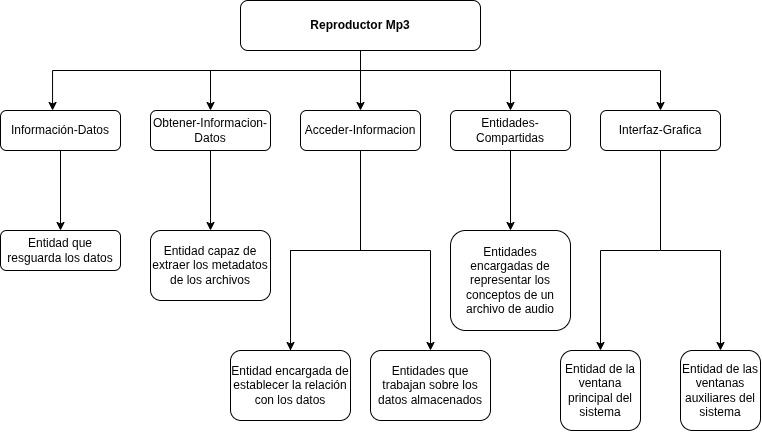
\includegraphics[width=1\textwidth]{analisis.jpg}
    \caption{Diagrama de los módulos con sus entidades del sistema.}
    \label{fig:protocolo}
\end{figure}

\vspace{0.5cm}

\noindent Como podemos ver en el diagrama, hemos logrado identificar los problemas y subproblemas principales a los cuales nos enfrentaremos a lo largo del desarrollo de este sistema. Este análisis se hizo de la manera más abstracta posible, pues el objetivo de este paso, es idear una solución sin adentrarnos del todo con las tecnológias particulares que serán necesarias de usar.

\vspace{0.2cm}

\noindent Del análisis podemos identificar una cosa frecuente, las cuáles son las entidades. Tenemos entidades que realizan una acción en partícular con una responsabilidad única, por tanto podemos encontrar factible implementar este sistema con una solución enfocada al paradigma orientado a objetos, pues cada entidad que hemos definido en nuestro análisis podría ser modelada con un objeto, que, en su conjunto nos ayudará a poder desarrollar el sistema de  Reproductor mp3.

\vspace{0.2cm}

\noindent Por tanto, una vez que elegimos el paradigma con el que trabajaremos, y apoyandonos en gran medida con el diagrama que obtuvimos al realizar el análisis del problema, podemos pasar a la siguiente parte del desarrollo, la cual consiste en diseñar una solución con base en nuestro análisis.

\vspace{0.5cm}



\chapter{Diseño de la solución al problema}

\noindent Ahora es donde analizaremos como llevar nuestro análisis a una solución que podamos aplicar de manera partícular para la resolución de nuestro problema.

\vspace{0.2 cm}

\noindent Es por ello que ahora si es necesario hablar de las tecnológias requeridas, así como hablar de la especificación que se nos dio para realizar nuestro sistema.
Se nos proporcionó un esquema sql el con el cuál construiremos una base de datos donde vivirán los datos del programa. Las tablas del esquema son las siguientes: \textit{types, performers, persons, groups, in\_group, albums, rolas}.

\vspace{0.2cm}

\noindent Por tanto vemos que de cada archivo archivo de audio que recibamos deberemos de extraer los metadatos correspondientes para poder llenar nuestra base de datos.

\noindent La base de datos se trabajará con Sqlite, esta decisión se toma pues necesitamos (y se nos pidió) hacer uso de una base de datos relacional, por tanto Sqlite se ajusta a dicha necesidad, además de que por ahora no es necesario levantar un servidor donde viva la base de datos, por tanto un archivo \textit{.db} donde resida la base de datos es una decisión pertinente.

\vspace{0.2cm}

\noindent La discusión anterior nos hace relacionar que la base de datos será parte de nuestro módulo \textit{Información-Datos}, que justamente habiamos planteado como el lugar donde se resguardarán los datos recolectados de los archivos de audio, por tanto pasaremos a llamar a ese módulo como \textit{Base de datos}.

\vspace{0.5 cm}

\noindent Ya tenemos clara la tecnológia con la que trabajeremos para almacenar los datos, por tanto el siguiente paso es saber como es que vamos a estructurar nuestro sistema. Vemos que cada módulo definido en el análisis tiene una responsabilidad única, que si bien puede tener conexiones con los otros módulos ,la lógica de cada uno de ellos sólo se queda en el módulo en donde vive; vemos que por la manera en que estan definidos los módulos es natural pensar en el patrón de diseño Modelo-Vista-Controlador (\textit{MVC}), veamos la justificación:

\vspace{0.2cm}

\noindent Tenemos que el módulo \textit{Base de datos} resguardará nuestra base de datos a la cuál tendremos acceso durante la ejecución del programa, pero debe de haber alguna manera en la cual podamos acceder a dicha base de datos, por tanto los módulos \textit{Obtener-Informacion-Datos, Acceder-Informacion, Entidades-Compartidas} son los encargados de hacer las operaciones necesarias sobre la base de datos. Vemos que dichos módulos se ajustan de manera correcta a la parte del Módelo de \textit{MVC}, pues justamente es en ellos donde vive la lógica del negocio encargada de manejar los datos; Por tanto ajustando nuestro análisis a \textit{MVC} tenemos cubierta la parte del módelo.

\vspace{0.2cm}

\noindent Ahora bien, no hay que olvidar que debemos de desarrollar una manera para que el usuario pueda tener interacción con el programa, justamente (cómo habíamos definido en el análisis) el módulo \textit{Interfaz-Grafica} es el encargado de dicha tarea, pues es aquí donde vivirá la forma en la cuál se le presentará información al usuarim justamente si acoplamos esto al patrón \textit{MVC} cumple con las características que la parte de Vista espera tener; de esa manera, dicho módulo lo pasaremos a renombrar como \textit{Vista}.

\vspace{0.2cm}

\noindent Bien, ya que tenemos definido con base en nuestro análisis tanto al modelo como la vista, nos falta la capa del controlador; sabemos que el controlador en grandes rasgos se encargá de gestionar la relación que tenemos entre nuestro modelo y nuestra vista, vemos que en nuestro análisis no tenemos algún módulo que se pueda adaptar al controlador, por tanto por ahora basta definir que el controlador hara llamadas a las operaciones definidas en los objetos de nuestro modelo, que sirva como puente que se le pueda pasar a la vista, por tanto, no es que en este caso el controlador implemente lógica nueva, por ello es que se hizó omisión de este en el análisis pues es un módulo o capa que debía de ser definido ahora que estamos pensando en tecnólogias particulares; de esa manera, es que podemos definir una nueva capa llamada \textit{Controlador}

\vspace{0.2cm}

\noindent Por tanto tenemos una primera versión del diagrama de \textit{MVC} 

 \begin{figure}[H]
    \centering
    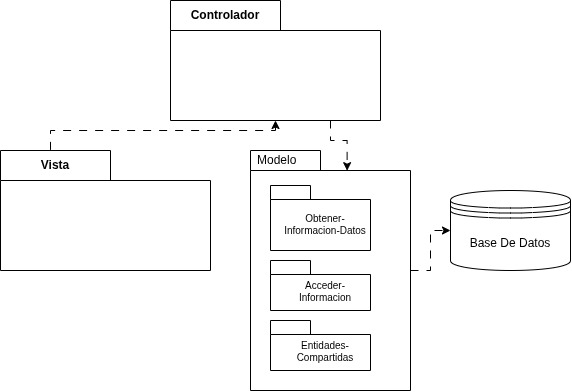
\includegraphics[width=0.55\textwidth]{Mvcinicial.jpg}
    \caption{Diagrama inicial de MVC.}
    \label{fig:mvcInicial}
\end{figure}

\noindent 

\vspace{0.5cm}

\noindent Sigamos dando forma a nuestro diseño; por ahora solo estamos definiendo que módulos formarán parte de nuestro \textit{MVC}, por tanto vemos que el la única capa que tiene subcapas es el \textit{Modelo}, por tanto haremos una refactorización en los nombres de cada subcapa para que de esa manera podamos tener una mayor claridad sobre su responsabilidad.

\vspace{0.2cm}

\begin{itemize}
    \item [-] \textit{Obtener-Informacion-Datos}\\
    Como discutimos en el análisis este módulo se encarga de obtener los datos de los archivos de audio, para poder llenar nuestra ahora llamada \textit{Base de datos}. Si vamos a la especificación proporcionada, un requerimento que se pide es tener un minero que recorra un directorio proporcionado que analice archivos mp3 con etiqueta Idv3v2.4, justamente desde un inicio este módulo fue pensado para cumplir con dicha funcionalidad, por tanto es en este momento que podemos pasar a renombrarlo como \textit{Minero}.
    
    \item [-] \textit{Acceder-Informacion}\\
    \noindent Este módulo ahora hablando de manera menos generalizada, como habiamos mencionado seŕa el encargado de acceder a la base de datos para ejecutar operaciones/consultas sobre la misma, por tanto lo renombraremos como \textit{AccesoDatos}

    \item [-] \textit{Entidades-Compartidas}\\
    \noindent Este módulo ya es descriptivo en su nombre, pero ahora que ya podemos hablar de tecnólogias específicas, vemos que, dado que estamos trabajando con el paradigma orientado a objetos, es en este módulo donde representaremos a las tablas que conforman nuestra base de datos (como rola, album o performer) como objetos en nuestro sistema; por tanto simplemente pasaremos a renombrar este módulo como \textit{Entidades}
\end{itemize}

\vspace{0.2cm}

\noindent Con dichos cambios realizados tenemos el siguiente diagrama de \textit{MVC} 

 \begin{figure}[H]
    \centering
    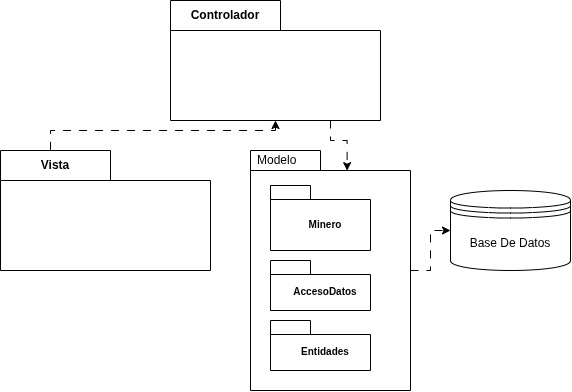
\includegraphics[width=0.8\textwidth]{Mvc2.jpg}
    \caption{Diagrama de MVC.}
    \label{fig:mvc}
\end{figure}



 \vspace{0.5cm}
 
 \noindent Ahora, como siguiente parte de la parte de diseño, pasaremos a definir como van a estar construidas las capas de nuestro modelo, sin olvidar el análisis que hicimos previamente.

 \vspace{0.5cm}

\noindent \textbf{Modelo: Entidades}

\noindent Hemos discutido que esta capa es la encargada de representar los metadatos extraídos de una archivo de audio como objetos. Como dichos objetos estan estrechamente relacionados con la información que representa las tablas en la base de datos, este módulo quedará conformado por los siguientes objetos:

\begin{itemize}
    \item [-] \textit{Rola}: Este objeto modela al archivo Mp3, por tanto siguiendo la especificación de la tabla de \textit{rolas} podemos obtener los siguientes atributos del objeto: \textit{id\_rola, album, performer, path, title, track, year, genre}
    \item [-] \textit{Performer}: Este objeto modela al interprete de una rola, por tanto siguiendo la especificación de la tabla de \textit{performers} podemos obtener los siguientes atributos del objeto: \textit{id\_performer, id\_type, name}
    \item [-] \textit{Album}: Este objeto modela al album de una rola, por tanto siguiendo la especificación de la tabla de \textit{albums} podemos obtener los siguientes atributos del objeto: \textit{id\_album, path, name, year}
    \item [-] \textit{Person}: Este objeto modela a una persona, que es uno de los tipos que puede ser un interprete, por tanto siguiendo la especificación de la tabla de \textit{person} podemos obtener los siguientes atributos del objeto: \textit{id\_person, stage\_name, real\_name, birth\_date, death\_date}
    \item [-] \textit{Group}: Este objeto modela a un grupo, que es uno de los tipos que puede ser un interprete, por tanto siguiendo la especificación de la tabla de \textit{group} podemos obtener los siguientes atributos del objeto: \textit{id\_group, name, start\_date, end\_date}
\end{itemize}

\noindent Tenemos los objetos principales con los cuales estaremos trabajando durante la elaboración de nuestro programa, sin embargo debemos tomar que en principio, al obtener los metadatos de un archivo de audio, dichos datos no es que automaticamente sean capaces de modelar a nuestros objetos con precisión, por tanto es importante pensar en un objeto que sirva como ``base`` de la cual nos apoyaremos para poder raestrear la información de mejor manera, a dicho objeto le llamaremos \textit{DatosMp3}.

\begin{itemize}
    \item [-] \textit{DatosMp3}: Este objeto sirve como la base la cua recibirá la información ``cruda`` de los archivos de audio, por tanto definimos los siguientes atributos: \textit{titulo, artista, album, track, anio, generos, ruta, versionId3}
\end{itemize}

\noindent Por tanto el diagrama de clases de la capa de \textit{Entidades} del \textit{Modelo} se ve de la siguiente manera:

 \begin{figure}[H]
    \centering
    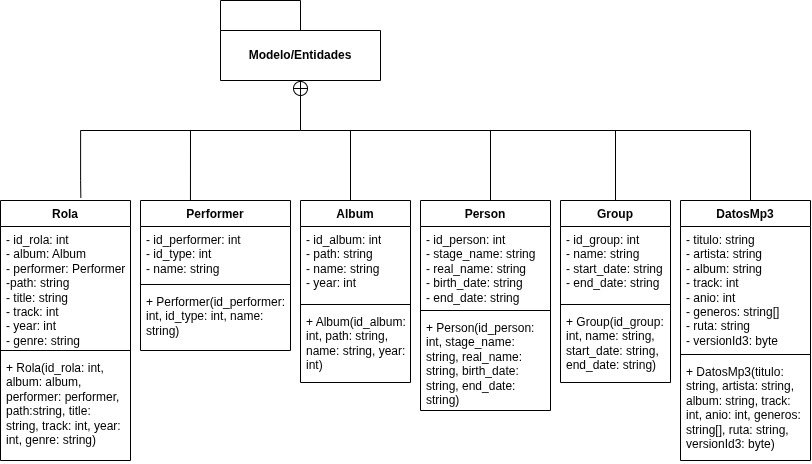
\includegraphics[width=1.2\textwidth]{Entidades.jpg}
    \caption{Diagrama de la capa \textit{Entidades}.}
    \label{fig:Entidades}
\end{figure}

\noindent \textbf{Modelo: Minero}

\noindent En ese módulo es donde nosotros albergaremos la lógica sobre como es que vamos a obtener los datos de los archivos de audio que nos pasen mediante un directorio especificado, para poder resguardarlos en nuestra base de datos; vemos que dicha función la podemos realizar al definir un solo objeto, al cual le llamaremos \textit{MineroMp3}.

\begin{itemize}
    \item [-] \textit{MineroMp3}: Este objeto como ya hemos mencionado, contiene la lógica por la cual accedemos y guardamos los metadatos de cada archivo, por tanto definiremos la operaciones para poder realizar dicha función.

    \begin{itemize}
        \item [-] \textit{GuardarArchivosMp3}: Esta operación tiene como finalidad que, dado un directorio especificado, recorrerlo (así como sus subdirectorios) obtener los archivos con terminación ``.mp3`` y guardarlos en alguna estructua de datos adecuada.

        \item [-] \textit{AnalizarArchivoMp3}: Esta operación tiene como fin, que dado una ruta de un archivo de audio con terminación \textit{.mp3}, obtener los metadatos del archivo para así formar un objeto de tipo \textit{DatosMp3} que nos servirá como base para poder crear los objetos con los cuales llenaremos nuestra base de datos. Cabe señalar que aquí sería conveniente poner una restricción sobre los archivos que vale la pena analizar, pues deberán de cumplir con tener por lo menos la etiqueta Id3v2.

        \item [-] \textit{VerificarVersionId3}: Esta operación nos ayudará a poder verificar que la versión de la etiqueta de un objeto de \textit{DatosMp3}, que construímos con el archivo de audio, sea la correspondiente con la que se nos pide en la especificación que es Id3v2.4

        \item [-] \textit{MinarDirectorio}: Esta es la operación principal de nuestro objeto, ya que las anteriores fueron definidas para poder hacer que esta operación este bien construida, lo que haremos en esta operación es que dado un directorio, obtengamos una estructura de datos que contendra datos de tipo \textit{DatosMp3}, que se va a construir con los metadatos de los archivos de audio rescatados de las operaciones auxiliares \textit{GuardarArchivosMp3} y \textit{AnalizarArchivosMp3}

        
    \end{itemize}
\end{itemize}

\noindent Por tanto el diagrama del módulo minero lo podemos ver de la siguiente manera:

 \begin{figure}[H]
    \centering
    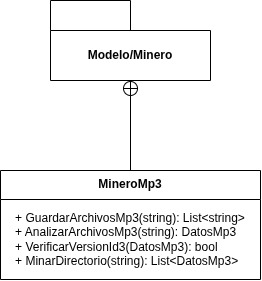
\includegraphics[width=0.4\textwidth]{Miinero.jpg}
    \caption{Diagrama de la capa del Minero.}
    \label{fig:Minero}
\end{figure}

\noindent \textbf{Modelo: AccesoDatos}

\noindent En este módulo recordemos que habíamos definido en nuestro análisis; en nuestro análisis aquí habíamos definido dos agentes involucrados: una entidad que se encargue de realizar nuestra conexión a nuestra base de datos, y entidades que se encargarán de trabajar sobre los datos almacenados en la base de datos. Hagamos enfásis por ahora en el objeto encargado  de realizar la conexión, al cual le llamaremos \textit{ConexionBaseDeDatos}.

\begin{itemize}
    \item [-] \textit{ConexionBaseDeDatos}: Este objeto se encargará de conectar nuestro sistema con la base de datos, necesitamos que dicha conexión sea única, pues cada vez que hagamos uso de este objeto no necesitamos crear una nueva conexión, sino que acceder a la misma conexión en todo momento; vemos que dichos requerimentos se acoplan de manera natural al patrón de diseño \textit{Singleton}, pues recordando que este patrón garantiza que un objeto tenga una única instancia en toda la aplicación ademas de que proporciona un punto de acceso global a dicho objeto, es justo lo que necesitamos para poder modelar dicho objeto; así siguiendo este patrón de diseño podemos definir como atributo a: \textit{conexionBaseDeDatos} que es un atributo de el mismo.
    Ademas vemos que las operaciones de este objeto  son:

    \begin{itemize}
        \item [-] CrearConexion: Esta operación será la encargada de crear la conexión con nuestra base de datos, recordando en todo momento que estamos trabajando con Sqlite.
         \item [-] \textit{GetInstancia}: Esta operación será la encargada de controlar que cada vez que se quiera obtener un objeto de este tip, se devuelva siempre la misma instancia, así, si la instancia aún no eciste la crea; si ya existe, solamente la devuelve sin crear una nueva. 
    \end{itemize}

     \begin{figure}[H]
    \centering
    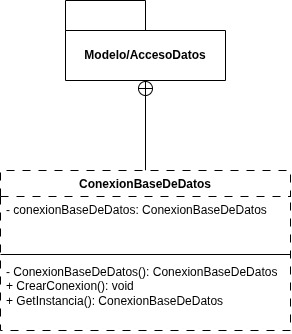
\includegraphics[width=0.4\textwidth]{Singleton.jpg}
    \caption{Diagrama de la capa del AccesoDatos Singleton}
    \label{fig:singleton}
\end{figure}
\end{itemize}

\noindent Ahora que ya definimos el objeto encargado de conectarnos con la base de datos, debemos de pensar en las entidades que se encargarán de trabajar sobre los datos de la base de datos. Es aquí donde vamos a definir las consultas que se harán a la base de datos; Este tipo de entidades las vamos a abordar aplicando el patrón de diseño \textit{Data Access Object (DAO)}, vemos que este patrón se ajusta de manera adecuada pues separamos la lógica de como accedemos a los datos con la lógica del negocio; vemos que cada DAO se encarga de realizar las operaciones de consulta en SQL, donde podemos aplicar las operaciones estándar que nos da este patrón de diseño, las cuales son las llamadas \textit{CRUD (Create, Read, Update, Delete)} y asi encargarnos de convertir resultados de la base de datos y viceversa. Por tanto es aqui donde tambien haremos uso de la capa de \textit{Entidades} pues dichas entidades fueron definidas con base en la especificación de la base de datos que recibimos,  por tanto resulta lógico que cada entidad tenga su propio \textit{DAO} para poder hacer la relación con la base de datos.

\vspace{0.2cm}

\noindent Vemos que el patrón define las operaciones mediante una interfaz, por tanto cada entidad tendra tanto su \textit{DAO} como su \textit{DAOImpl} que será la implementación de dicha interfaz; por tanto definimos los siguientes objetos: \textit{RolaDAO, PerformerDAO, AlbumDAO, PersonDAO, GroupDAO}.

\noindent Vemos que en esta ocasión no desglozamos cada objeto pues todos van a compartir como base las operaciones \textit{CRUD}.

 \begin{figure}[H]
    \centering
    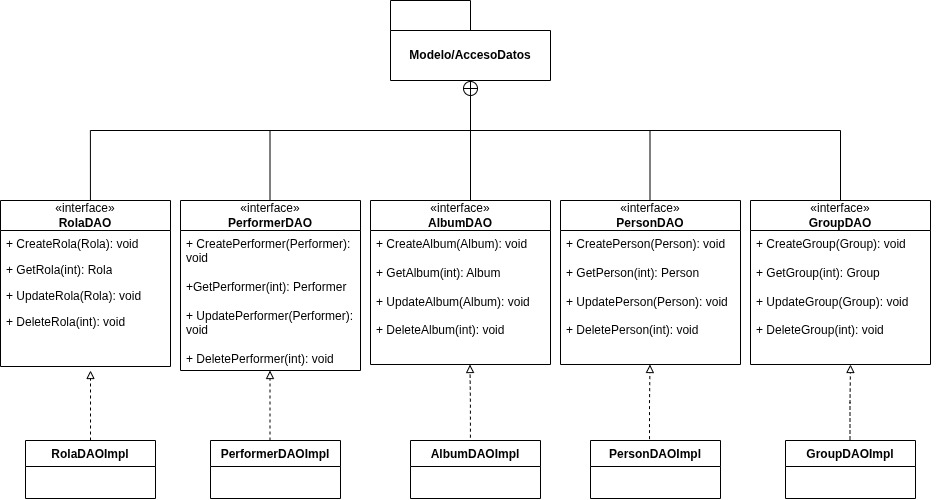
\includegraphics[width=1\textwidth]{Daos.jpg}
    \caption{Diagrama de la capa del AccesoDatos DAO´s}
    \label{fig:daos}
\end{figure}
 
\vspace{0.6cm}



\noindent De esa manera queda definido el diseño de nuestra capa de \textit{Modelo}, por tanto ahora hablaremos de la capa del controlador, que será la encargada del puente entre nuestra lógica de negocio con nuestra vista.

\vspace{0.5cm}

\noindent \textbf{Controlador}

\noindent Vemos que esta capa no la tenemos definida como algún módulo de nuestro análisis, sin embargo ahora contamos con las herramientas para poder definir de mejor manera esta parte del patrón de diseño \textit{MVC}.

\vspace{0.2cm}

\noindent Sabemos que esta capa es la encargada de coordinar el  intercambio de información entre la interfaz y el resto del sistema por tanto con base a recurrir a nuestra manera de acceder a los datos con nuestro patrón de diseño \textit{DAO}, resulta natural que en esta capa vivan objetos que llamen de manera directa a las operaciones de los \textit{DAO} de nuestro modelo, así dejandolos expuestos para poder ser llamados en nuestra capa de \textit{Vista}; por lo anterior podemos definir a los siguientes objetos:

\begin{itemize}
    \item [-] \textit{RolasControlador}: Expone las operaciones definidas en \textit{RolaDAO} necesarias para coordinarse con la capa \textit{Vista}
    
    \item [-] \textit{PerformerControlador}: Expone las operaciones definidas en \textit{PerformerDAO} necesarias para coordinarse con la capa \textit{Vista}
    
    \item [-] \textit{AlbumControlador}: Expone las operaciones definidas en \textit{AlbumAO} necesarias para coordinarse con la capa \textit{Vista}
    
    \item [-] \textit{PersonaControlador}: Expone las operaciones definidas en \textit{PersonDAO} necesarias para coordinarse con la capa \textit{Vista}
    
    \item [-] \textit{GrupoControlador}: Expone las operaciones definidas en \textit{GrupoDAO} necesarias para coordinarse con la capa \textit{Vista}
\end{itemize}

 \begin{figure}[H]
    \centering
    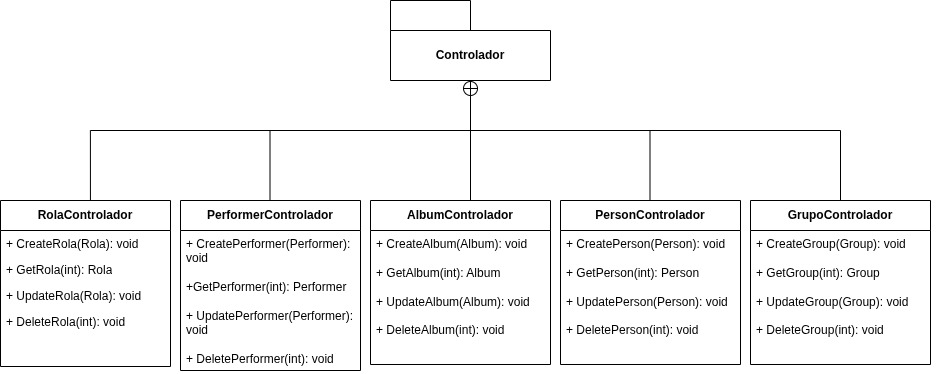
\includegraphics[width=1\textwidth]{daoControlador.jpg}
    \caption{Diagrama de la capa del controlador entidades}
    \label{fig:daos}
\end{figure}

\noindent Así tenemos definida una gran parte de esta capa \textit{Controlador} sin embargo, no debemos de olvidar una pieza importante en esta parte del sistema; en el modelo, siendo más especificos, en el módulo \textit{Minero} tenemos el objeto \textit{Minero} el cual por ahora solo se encarga de rescatar la información de los archivos de audio como una lista de objetos que podemos manejar su lógica en el sistema, por tanto es aquí donde definiremos como trabajar con dichos objetos para poblar de manera adecuada nuestra base de datos; así, definimos al objeto \textit{MineroControlador}.

\begin{itemize}
    \item [-] \textit{MineroControlador}: Este objeto tiene como finalidad conectar la información que rescatamos de los archivos de audio con la base de datos, por tanto podemos pensar en los siguientes atributos del objeto: \textit{minero, performerDAO, albumDAO, rolaDAO}. Ahora pasamos a definir las operaciones:

    \begin{itemize}
        \item [-] \textit{MinarDirectorio}: Esta operación tiene como finalidad que dado un directorio que reciba como entrada, minar dicho directorio haciendo uso del minero, para posteriormente guardar la información en una estructura de datos siempre y cuando cumpla con la especificación de que la etiqueta Id3 del archivo sea la versión 2.4
        \item [-] \textit{ObtenerOCrearPerformer}: Esta operación nos ayuda a determinar si el performer que estamos pasando como entrada ya existe como un registro en la base de datos, pues si existe solo lo devuelve, y en caso de no hacerlo, hace uso de performerDAO para agregar al performer al registro en la base de datos. 
        
        \item [-] \textit{ObtenerOCrearAlbum}: Esta operación nos ayuda a determinar si el album que estamos pasando como entrada ya existe como un registro en la base de datos, pues si existe solo lo devuelve, y en caso de no hacerlo, hace uso de albumDAO para agregar al performer al registro en la base de datos. 

        \item [-] \textit{GuardarDatos}: Esta operación es la que nos permitirá guardar los datos que nos lleguen de un archivo de audio, en la base de datos, pues aquí se piensa hacer uso de los atributos objeto \textit{DatosMp3} que pasaremos como entrada, para crear objetos de tipo Rola, Performer y Album que se mandarán a guardar en la base de datos. Es por ello que se definieron las operaciones anteriores, para guardar una relación entre el interprete y el albúm asociado a la Rola.  

        \item [-] \textit{MinarYGuardar}: Esta operación es la que se encargará de hacer el minado completo, pues hace uso de operaciones como \textit{MinarDirectorio} la cual nos devuelve datos validos de los archivos de audio, para posteriormente mandar a guardar dichos datos a la base de datos con \textit{GuardarDatos}. Asi obteniendo un minado exitoso con los metadatos de los archivos de audio que cumplen con la especificación requerida.
    \end{itemize}
\end{itemize}

 \begin{figure}[H]
    \centering
    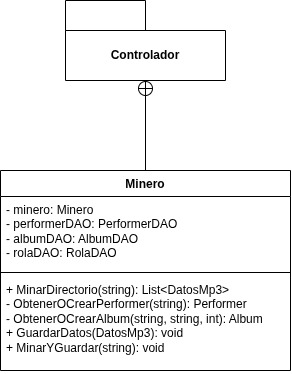
\includegraphics[width=0.4\textwidth]{mineroControlador.jpg}
    \caption{Diagrama de la capa del controlador/minero}
    \label{fig:mineroControlador}
\end{figure}

\noindent Hemos definido de manera satisfactoria a la capa del controlador, por tanto, la última capa a definir es la de la \textit{Vista}

\vspace{0.5cm}

\noindent \textbf{Vista}
En esta capa, debemos de preocuparnos la manera en que mostramos la información al usuario final, esta etapa de manera ideal lo único que hace es relacionarse con el controlador del sistema para permitir un intercambio de datos entre los diferentes módulos que tiene nuestro sistema. Por tanto, podemos definir a esta capa, no que haga uso de objetos, sino como ventanas del sistema que se le muestran al usuario; asi las ventanas que podemos definir para la parte de la vista son las siguientes: 

\begin{itemize}
    \item [-] \textit{VentanaPrincipal}: Es aquí donde se planea mostrar la información mas relevante del sistema al usuario, como la lista de canciones, una manera de reproducirlas, y donde podremos acceder a las diferentes ventanas que el programa podrá contenter.
    \item [-] \textit{VentanaBusquedaAvanzada}: Dado que un requerimento del sistema es el poder realizar búsquedas avanzados, tener una ventana enfocado a ello resulta buena idea, pues hace que el programa sea más intuitivo.
    \item [-] \textit{VentanaMostarAlbums}: Si bien en la ventana principal mostramos información relacionada a las rolas, tener una ventana la cuál nos presente la información de los albums resulta una decisión lógica de diseño.
    \item [-] \textit{VentanaMostrarPersons}: Mismos argumentos que en VentanaMostarAlbums.
    \item [-] \textit{VentanaMostrarGroups}: Mismos argumentos que en VentanaMostarAlbums.
    
\end{itemize}

 \begin{figure}[H]
    \centering
    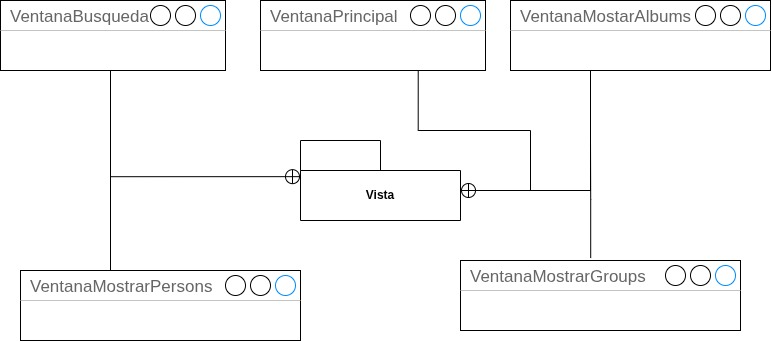
\includegraphics[width=0.9\textwidth]{vistas.jpg}
    \caption{Diagrama de la capa del vista}
    \label{fig:vista}
\end{figure}

\vspace{0.2cm}

\noindent Ya hemos definido cada capa del sistema, por tanto ya tenemos un diseño factible que podemos seguir para pasar a la implementación del diseño; por tanto pasaremos a la siguiente etapa del reporte.

    \chapter{Implementación del diseño}

    \noindent En esta etapa del desarrollo del sistema es donde vamos a darle vida a nuestro diseño dado, es decir, es la etapa de la programación; nuestro diseño lo modelamos de tal manera que debería de ser reproducible sin necesidad de estar ligado con algún lenguaje de progrmación, pero claramente para este proyecto fue necesario elegir alguno, por tanto como primer punto pasaremos a explicar el lenguaje de programción.

    \vspace{0.2cm}

    \noindent \textbf{Lenguaje de programación}

    \noindent Para desarrollar este proyecto se busco en primer instancia un lenguaje que nos permitiera trabajar de manera natural con el paradigma de orientación de objetos; lo anterior nos una lista predefinida de ciertos lenguajes como \textit{Java, C++, C\#} entre otros. Sabemos que tenemos una restricción para \textit{Java} por tanto no figura como posibilidad real, asi tenemos dos opciones fuertes, las cuales son \textit{C++} o \textit{C\#}. 
    La decisión entre ambas es una decisión crucial, pues si bien ambas pueden compartir la orientación a objetos, tienen ciertas diferencias que nos pueden facilitar o dificultar el desarrollo del proyecto

    \begin{itemize}
        \item [-] \textit{C++}: Vemos que C++ nos ofrece la orientación a objetos, además de un punto importante. Dado que el sistema debía contar con una interfaz gráfica, esto nos permitia pensar en programas como \textit{Qt} o \textit{GTK}; \textit{Qt} es un sistema la cuál su lógica principal esta construída en \textit{C++}, por tanto si desarrollaramos la parte del modelo y el controlador en \textit{C++}, esto nos permitiría un acoplamiento de manera natural con la vista. Por lo anterior, puede parecer que \textit{C++} es una decisióm factible, sin embargo ofrece dificultades para mi, pues no estoy relacionado con dicho lenguaje, además de su parecido con \textit{C} crea una gran barrera la cual me hace descartar dicha opción a pesar del punto fuerte que contiene este lenguaje.
         \item [-] \textit{C\#}: Por otro lado, \textit{C\#} es un lenguaje que esta tambien basado en el paradigma orientado a objetos, además de que este lenguaje comparte una estructura muy parecida a la de \textit{Java}, este es un punto fuerte, pues la experiencia que tengo como programador es pincipalmente en \textit{Java}, por tanto desarrollar usando un lenguaje parecido \textit{Java} es una característica de gran valor para mi; tambien dado que durante el proyecto 1 obtuve experiencia usando \textit{C\#} volver a elegirlo como lenguaje de programación principal parece buena opción; sin embargo no todo es color de rosa, pues aún debemos de resolver como desarrollar la \textit{GUI}, pues \textit{GTK} se apoya en \textit{C} mientras que \textit{Qt} se apoya en \textit{C++}, por tanto intentar acoplar alguna de las dos a \textit{C\#} es una dificultad añadida al proyecto, pero que desde mi punto de vista no es algo que nos haga perder tanto respecto a las ventajas que ganamos al usar \textit{C\#}.
    \end{itemize}

    \noindent Por los argumentos anteriores es que se decidió usar \textit{C\#} como lenguaje de programación,

    \vspace{0.5cm}

    \noindent \textbf{Manera en que se manejará la interfaz gráfica}

    \noindent Durante las discusiones acerca del proyecto en las horas de clase, se nos dierón opciones sobre como manejar el desarrollo de la interfaz gráfica, ,opciones como \textit{Qt, Gtk} e incluso \textit{JavaFX}, fueron algunas de las mencionadas. 

    \vspace{0.2cm}
    
    \noindent \textit{JavaFX} no llego a ser considerada, dado que si bien, al parecer puede ser usada sin necesidad de trabajar con el lenguaje \textit{Java}, preferí ahorrarme las dificultades que podría llegar a haber al querer conectarlo con la lógica desarrollada en \textit{C\#}.

    \vspace{0.2cm}

    \noindent Ahora bien, \textit{GTK} esta pensado para trabajar en \textit{C}, y esa es razón suficiente para no ser considerado.
    
    \vspace{0.2cm}

    \noindent Por tanto nos quedamos como única opción para trabajar con \textit{Qt}. Cómo primera instancia esto es una dificultad, pues el único framework con el que he trabajado ha sido \textit{Avalonia} utilizado en el proyecto del chat, y realmente no fue algo espectacular, pues en esencia, dicho proyecto se construyo usando cosas muy básicas como cajas de texto y botones; sin embargo, esta interfaz gráfica debería de contenter más elementos, como tablas dinámicas e incluso una manera de reproducir un archivo.

    \noindent \textit{Qt} por si mismo nos puede ayudar de sobremanera en ello; una de sus herramientas que nos ayudó a desarrollar el ssitema fue \textit{QtCreator} la cuál nos permite dibujar la interfaz gráfica arrastrando los elementos a la pantalla, generando de manera automática el código en formato \textit{qml} sin necesidad de ir escribiendo linea por linea dicho código, que aún con ello no nos libramos del todo, pues para hacer que los elementos de la interfáz gráfica fueran dinámicos con el tamaño de la pantalla si fue necesario escribir código \textit{qml} para cumplir con dicha necesidad.

    \vspace{0.2 cm}
    
    \noindent Fue gracias a esta herramienta que las ventanas planeadas en el diseño se pudieron diseñar con relativa facilidad, o al menos el esqueleto de las mismas; cabe destacar que durante el desarrollo, nos dimos cuenta que fue necesario diseñar más ventanas de las pensadas, pero dichas ventanas nos sirvieron para poder hacer una experiencia de usuario más amigable, pues fue conforme se iba probando el programa que se veía en la necesidad de definir nuevas ventanas para ser más claros en las funcionalidades del programa.

    \vspace{0.2cm}

    \noindent De la manera que lo mencionamos fue que definimos e implementamos los esqueletos de las ventanas, sin embargo ahora toca explicar como es que logramos exponer nuestra lógica construída en \textit{C\#} a la vista.

\noindent Al inicio donde buscamos que opciones se tenían para exponer la lógica se considero una idea de impementar un protócolo de comunicación mediante \textit{Json} para poder comunicar la lógica del negocio en el lenguaje \textit{C\#} con la vista en \textit{C++}. Esta idea surgió de la necesidad de exponer el controlador y el módelo a la vista, pues algo parecido hicimos en el primer proyecto, pero pronto se vió que esto era agregar un nivel de dificultad innecesariamente complejo, por tanto se debía de buscar alguna otra ruta. 

\vspace{0.2cm}

\noindent La ruta que seguimos fue usar el framework \textit{Qt bridge for C\#}, el cuál nos permite conectar una lógica de aplicación escrita en \textit{C\#} con una interfaz gráfica construida en \textit{Qt} con \textit{qml}. No hay manera de describir el asombró e impresión al descubrir dicha manera de hacer la conexión, por que más alla de que nos ayudó de manera ENORME en la realización del proyecto, lo impresionante es que este proyecto de \textit{Qt bridge} aún no esta lanzado de manera oficial pues se probó una versión beta que apenas fue lanzada en mayo de este mismo año, es decir que durante este proyecto se implementó una tecnológia que apenas esta en desarrollo, lo cual de manera genuina se me hace sorprendente pues sin esta solución no se que otra ruta habría tomado este proyecto.

\vspace{0.2cm}

\noindent Usar dicho framework fue tan sencillo como simplemente hacer una instalación usando \textit{dotnet} que nos generó automaticamente la base para poder trabajar sobre el mismo.
\noindent La manera en que conectamos la lógica del negocio fue que se tuvó que implementar clases que sirvieran como puente entre el controlador y nuestras ventanas en \textit{qml} , dichas clases basicamente solo contienen llamadas a los métodos del controlador, así respetando el patrón \textit{MVC}; lo anterior se hizó, pues ya que \textit{qml} lo podemos ver como un lenguaje declarativo, es posible declarar funciones dentro del archivo qml, que a su vez dichas funciones hacen llamadas a los métodos de la clases puente, así permitiendo que dentro de la misma interfaz podamos hacer uso de operaciones como minar un directorio, o editar datos que se guarden en la base de datos, por mencionar algunos.

\vspace{0.2cm}
\noindent Así resumiendo esta parte, la manera en que diseñamos la interfaz gráfica fue usando \textit{Qt} con el framework \textit{Qt bridge for C\#}.

\vspace{0.5cm}

\noindent \textbf{Algunas funcionalidades del programa}

\noindent Esta sección explica las funcionalidades que podrían no ser explicitas en la ejecución del programa.

\begin{itemize}
\item [-] ¿Cómo editar los datos de una canción? : Cuando ejecutamos el programa, vemos que se llena nuestra tabla con las canciones minadas y se muestran los datos, como tenemos referencia a las celdas de la tabla, basta con dar doble click en el dato que quieras cambiar, escribir la nueva información, y dar \textit{enter} para así haber actualizado el dato. Esto funciona con las columnas: \textit{Nombre, Genero, Anio} 

\item [-] ¿Cómo editar los datos de un albúm? : Para actualizar los datos de un albúm es un proceso similar, solamente debemos ir a la ventana donde podemos observar los albúmnes, y una vez ahí, dar doble click sobre la celda del dato que quieras cambiar, escribir el dato y presionar \textit{enter} para realizar el cambio. Esto funciona con las columnas: \textit{Nombre, Año}.

\item [-] ¿Qué hace la barra de búsqueda?: La barra de búsqueda principal nos permite filtrar rolas por nombre, artsita, albúm, género, año e incluso si tenemos que una persona artista es integrante de un grupo, luego buscamos las rolas de ese artista tambien apareceran las rolas del grupo del cual el artista es integrante.

\item [-] Crear personas y grupos: Vemos que tenemos las ventanas para poder agregar personas y grupos, podemos agregar personas y grupos que no existen como performers en la base de datos, pero, si agregamos a una persona o a un grupo con el mismo nombre de un performer, ahora dicho performer se cambiará su tipo para asociarlo con una persona o con un grupo según corresponda.

\end{itemize}

\noindent Las funcionalidades explicadas anteriormente son aquellas que no quedan de manera explicita en el programa, por ello valia la pena explicarlas. Todo el resto de funcionalidades se intentarón hacer de tal manera que sean claras para un usuario que en primer instancia no tiene idea de como funciona el programa, por tanto omitimos la explicación de dichas funcionalidades.

\vspace{0.5cm}

\noindent \textbf{Sistema de construcción y documentacióm}

\noindent Para el sistema de construcción utilizamos \textit{Makefile} con el cuál ya habíamos trabajado anteriormente, pues este permite de manera muy sencilla ejecutar acciones con solo poner \textit{make}, es por ello que se decidió trabajar con dicho sistema de construcción

\vspace{0.2cm}

\noindent Para generar la documentación se hizó uso de \textit{DocFX}, no hay gran debate sobre el porqué se tomó dicha decisión, simplemente es una tecnológia que cumple con la función de generar la documentación de cada clase del código además de que nos la presenta en una página \textit{HTML} para una amigable navegación.



    \vspace{0.8cm}
    
    \chapter{Conclusiones}
    
    \noindent El desarrollo de este proyecto consideró que aporto un gran impacto en mi conocimiento sobre como desarrollar software, además de haber mostrado de mejor manera la razón de ser las etapas por las cuales se conforma el desarrollo, veamos la razón del porque digo esto.


    \vspace{0.2cm}

    \noindent Durante la introducción de este reporte se hizo mención a que gracias a las fallas que pudimos identificar en el primer proyecto, deberiamos de reflejar el aprendizaje en este nuevo proyecto, cosa que creo que se realizón con exito; lo anterior lo mencionamos debido a que al momento de atacar este nuevo problema se hizo un mayor enfásis la parte del modelado, pues durante el desarrollo del programa pocas veces se estuvó a la deriva, esto débido a que el diseño del problema se hizo de tal forma que cada parte a la que debíamos avanzar fuera natural de visualizar.

    \vspace{0.2cm}

    \noindent Sin embargo, por lo anterior es que ahora quedó un poco descuidada la parte de la implementación esto debido a que en retrospectiva hice mal en subestimar la etapa de la programación; expliquemos esto.

    \vspace{0.2cm}

    \noindent Como se hizó especial enfásis en el modelado, supuse que una vez que esté estuvo completo, la etapa de la progrmación resultaba ser sencilla, lo cuál fue un error, pues si bien mencionamos que en casi todo el proyecto sabíamos el camino a seguir y donde estabamos parados, realizar la implementación no resultaba sencilla, pues no es lo mismo definirlo de manera abstracta como lo hacemos en el diseño a llevarlo a una implementación real, pues por ejemplo al momento de tener que definir las consultas \textit{SQL} fue complicado, pues algunas no eran consultas triviales, esto se vió especialmente reflejado al momento de querer realizar parte de la búsqueda avanzada. 
    
    \noindent Sin embargo la parte que más considero subestimada fue la realización de la interfaz gráfica, pues incluso cosas como centrar un botón o hacer que el tamaño fuera dinámico fue complicado, pero no toda la complejidad fueron cosas técnicas; al momento de estar probando el programa, se empezó a ver la necesidad de definir nuevas pantallas, que por muy pequeñas que fueran, como una simple confirmación de alguna operación, se debía que recurrir a \textit{QtCreator} y dibujar la interfaz, para posteriormente aplicarla a todo el sistema, cosas de ese estilo que pueden ser considerados detalles, no los tome en cuenta, e incrementarón el tiempo que pense que sería necesario para desarrollar el proyecto.

    \vspace{0.5cm}

    \chapter{Referencias}

    \begin{itemize}
        \item [-] https://www.youtube.com/watch?v=yKcEDs1joXk
        \item [-] https://www.youtube.com/watch?v=9ldPFnu9iTY
        \item [-] https://www.qt.io/development/qt-framework/qt-bridges/csharp-gui?hsLang=en\#get-started
        \item[-] https://github.com/mono/taglib-sharp 
    \end{itemize}
\newpage



\vspace{1cm}
\end{document}